 \begin{center}
 \textbf{
 %\dots
\og 
\dots \og La Sainteté une voie ouverte à tous ! \fg{} \dots
 \fg{}
 %\dots
 }
 \end{center}

\begin{wrapfigure}{l}{2.2cm}
\vspace{-0.2cm}
	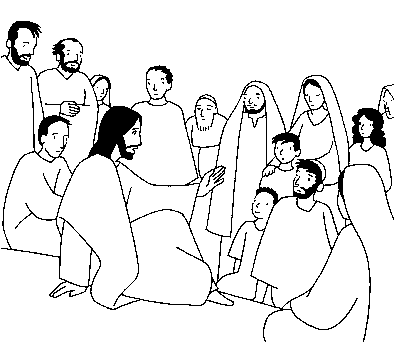
\includegraphics[scale=0.75]{../images/jesus_parle_foule}
\end{wrapfigure}
 Toute en étant une notion commune à toute les religions, la sainteté ne se définit pas de la même manière dans toutes les formes de spiritualité. Généralement, on considère comme sainte une personne qui a mené une vie exemplaire, qui a donc atteint un niveau assez élevé de communion avec Dieu et qui devient pour les autres un modèle. A ce niveau, la sainteté est l’aventure la plus belle que Dieu propose à chacun de nous. Elle n’est pas une utopie. Elle est tout simplement une participation à la vie même de Dieu. La sainteté est un appel à tous. Elle n’est pas réservée à une catégorie de personnes. Elle n’est pas non plus l’absence d’erreurs et de fautes. Elle est le fruit du regard d’amour du bon Dieu sur tous ses enfants. Le grand secret de la sainteté c’est l’amour. Ainsi, Le Christ notre frère nous a sauvé par sa mort et sa résurrection en nous communicant sa vie d’amour par le baptême. Et cette vie de baptême nous a rendu tous participants de sa sainteté.

\begin{wrapfigure}{l}{1.5cm}
\vspace{-0.2cm}
	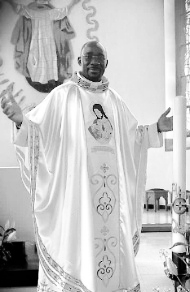
\includegraphics[scale=1.20]{../images/standing_daniel}
\end{wrapfigure}
En cette solennité de la Toussaint, disons-le, sans faut fuyant que la sainteté n’est pas un appel à la tristesse mais une vocation à la joie. Voilà pourquoi l’Evangile qui nous est proposé en cette fête revient plus d’une fois sur le vocable "heureux". Les saints se sont les bienheureux, ceux dont la vie est un rayonnement constant de joie, même au cœur de l’épreuve. \og Réjouissez-vous, soyez dans l’allégresse, car votre récompense sera grande dans les cieux. \fg{} Cette joie est celle de tous ceux qui nous ont précédés sur le chemin, et que nous célébrons aujourd’hui. Mais c’est aussi notre propre joie dès maintenant, encore discrète sans doute.

 Elle reste toutefois, une démarche qui s’enracine profondément dans l’humilité.


\begin{center}
Bonne fête de la Toussaint à toutes et à tous !!!
\end{center}


\begin{flushright}
\textit{Père  Daniel  ETTÉ}
\end{flushright}

